%============================================================================%
% Author: Pablo S�nchez                                                      %
%         p.sanchez@unican.es, http://personales.unican.es/sanchezbp         %
% Section : Motivation                                     Date: 25/02/2011  %
% Version : 1.0                                                              %
% Conference: SPLC 2011                                                      %
%============================================================================%

%============================================================================
% NOTE(Pablo): The angle of this section has changed
%============================================================================
%
% This section firstly introduces clonable
% features~\cite{czarnecki:2005d,czarnecki:2005} and explains the concepts
% and ideas behind them. Then, we explain why clonable features are
% important. Finally, we identify the research challenges created by
% clonable features.
%
%============================================================================

This section explains the shortcomings of feature modelling tools we faced during the development of a SmartHome SPL in the context of the AMPLE project. We comment on the research challenges we discovered and that we aim to solve in this paper.

\subsection{A feature model for a Smart Home SPL}

%============================================================================%
% Author: Pablo S�nchez                                                      %
%         p.sanchez@unican.es, http://personales.unican.es/sanchezbp         %
% Section : shortcomings                                   Date: 24/02/2011  %
% Version : 1.0                                                              %
% Conference: SPLC 2011                                                      %
%============================================================================%

\begin{figure*}[!tb]
  \includegraphics[width=\linewidth]{figures/FeatureModel.eps} \\
  \caption{Feature model for a SmartHome SPL}
  \label{fig:smartHomeFM}
\end{figure*}

%============================================================================
% NOTE (Pablo): This paragraph is left out for the SPLC 2011 version         
%============================================================================
%
% Let us consider the example presented in the previous section of the SmartHome 
% software product line. As commented before, a SmartHome can have a different
% number of floors and rooms. This kind of variability is called
% \emph{variability in structure}~\cite{sanchez:2007} and it can not be modelled 
% using traditional feature models~\cite{kang:1990}. Traditional feature models 
% can specify if a feature is mandatory or alternative, but not how many times a 
% feature can appear in a certain product.
% 
% This shortcoming can be solved using clonable features~\cite{czarnecki:2005}. A 
% \emph{clonable feature} is a feature that can appear with a variable number of times in 
% different products. A clonable feature is depicted like a normal feature but with a numerical % interval $[a..b] (a \ge b, b \in [0..*])$. This interval means that a product must appar at 
% least $a$ times and $b$ times as the maximum.
% 
% Feature models have experimented several evolutions in last decade. Recently, Czarnecki et 
% al~\cite{czarnecki:2005} introduced the simple but powerful concept of \emph{clonable 
% feature}. A clonable feature is a feature that can appear with a variable number of instances % in different products. A clonable feature is depicted like a normal feature but with
% a numerical interval $[a..b]$ above it. This interval means that a configuration of the 
% feature model must have at least % $a$ instances of this feature and $b$ instances at the 
% maximum. The upper bound can be $*$, which means there is no upper bound on the number of 
% instances.
%
% The upper bound can be $*$, which means there is no upper bound on the number of instances.
%
%============================================================================

Figure~\ref{fig:smartHomeFM} shows the feature model developed in the context of the AMPLE project for modelling a Smart Home SPL, based on a industrial case study provided by Siemens AG~\cite{ample:d52}\footnote{This feature model, as well as all the material presented throughout this paper, can be downloaded from \todo{URL TO BE PROVIDED}}. Clonable features were used in this case study to specify that an automated house can have several floors, with several rooms per floor. Each room can have a different number of devices, such as lights, heaters or windows, which can be automated.

The SmartHome SPL offers a set of services that can be included in the final software for a specific house. These services controls automatically a set of devices, such as windows, heaters or lights. Moreover, some advanced functions, such as Presence Simulation or Smart Energy Management, can be selected. This latter feature is on charge of coordinating windows and heaters to save energy. For instance, before heating a room, this feature will automatically close all the windows in that room to avoid wasting energy.

We would like to comment the feature model might be simplified by using \emph{feature references}~\cite{czarnecki:2005}. Feature references are often introduced in feature models to improve scalability  by means of avoiding redundancies. We might have created a feature model called \imp{Facilities} and to add \imp{LightMng}, \imp{WindowMng}, \imp{HeaterMng} and \imp{SmartEnergyMng} as subfeatures. Then, \imp{GeneralFacilities}, \imp{FloorFacilities} and \imp{RoomFacilities} would simply refer to \imp{Facilities}, avoiding replications. Although Hydra, our feature modelling tool, supports feature references, we have not used for this paper for the sake of simplicity, because they introduces some extra complexity in the explanations of the constraint analysis process which is not relevant for the purpose of this paper.

%============================================================================
% NOTE (Pablo): This paragraph is left out for the SPLC 2011 version
%============================================================================
% 
% It should be noticed that these houses can have, all of them, the same functionality; but 
% they can be different because they have a different structure, i.e., a different number of 
% instances of the features \imp{Floor}s and \imp{Rooms}. This kind of variability is called 
% \emph{variation in structure} or \emph{structural variability}~\cite{sanchez:2007}. Using
% traditional feature models without clonable features, this kind of variability can not be 
% properly captured, since  traditional feature models~\cite{kang:1990} can only express if a 
% certain feature or functionality is mandatory, optional or alternative, but not in what 
% number a certain feature can appear in a specific product.

%=================================================================================================================%
% TODO(Pablo): Add a some point of the text the semantics of references between features.                         %
%=================================================================================================================%

Figure~\ref{fig:smartHomeCfg} shows an example of configuration, or \emph{specialization}~\cite{czarnecki:2005e} of the feature model of Figure~\ref{fig:smartHomeFM}. 

The process of creating new instances of a clonable feature is called \emph{cloning}, and its semantics was clearly defined in Czarnecki et al~\cite{czarnecki:2005e}. This semantics specifies each time a new instance of a clonable feature is created, the subtree below the clonable feature is copied below this newly created feature. This subtree can then be configured as any other feature model. Changes in the subtree below an instance of a clonable feature have no influence on subtrees belonging to other instances. Therefore, each instance of a clonable feature can have its own configuration. To distinguish between different instances, or clones, of a same feature, we have opted for giving a different name to each instance. For instance, each instance of the \imp{Floor} feature has a different name (e.g. \imp{Ground}, \imp{First}), which indicates what floor is.

The configuration depicted in represents a simple house, with two floors - a ground floor and a first floor, and three rooms- a kitchen and a living room in the first floor and a bedroom in the first floor. Window Managament has been selected for the whole house; whereas LightMng is only selected for the Kitchen and the Bedroom. Heater and Smart Energy Management has been included in the living room. It should be noticed that the usage of clonable features allows a more fine-grained configuration of software products. Due to the use of clones for the different floors and rooms, we can customise each floor and/or room individually.

The reader could argue a Domain-Specific Language or Ecore model would be more useful for this case study than a feature. We will skip this question at this moment and we will come back to it in the discussion section. 

%============================================================================================
% NOTE(Pablo): This paragraph is better placed in a discussion section
%============================================================================================
% 
% This would not be possible using traditional feature models, where we need to create
% separate feature models for each floor and room and be responsible for manually managing 
% and synchronising them, which can be a cumbersome and error prone tasks. Using feature
%  models, these relationships are automatically specified and managed at the model level. For % instance, all feature models related to rooms of a same floor are subtrees of a same parent, % which is the clone for such a floor. For instance, all feature models related to rooms of a 
% same floor are subtrees of a same parent, which is the clone for such a floor.
% 
% , which would able to specify these facilities at the house, floor or room level. Therefore, % to create a model similar to the one depicted in Figure~\ref{fig:smartHomeFM}, we would
% have to create separate feature models for: (1) the whole house; (2) each individual floor;
% and (3) each individual room. This might lead to scalability problems, as we would need to
% manage a set of individual and unrelated feature models. Moreover, if some constraints, such % as ``if \imp{HeaterMng} is selected per house level, at least one \imp{Room} must contain a
% \imp{Heater}'', were defined, we would need to % manage different unrelated models at the
% same time in order to evaluate if this constraint is % satisfied or not. This can be a
% cumbersome and daunting task. Using clones, relationships between these different feature
% models are established. For instance, all feature models related to rooms of a same floor are % subtrees of a same parent, which is the clone for such a floor. This help to simplify the
% problem of evaluating the previously described constraint.
%
%============================================================================================

\begin{figure*}[!tb]
  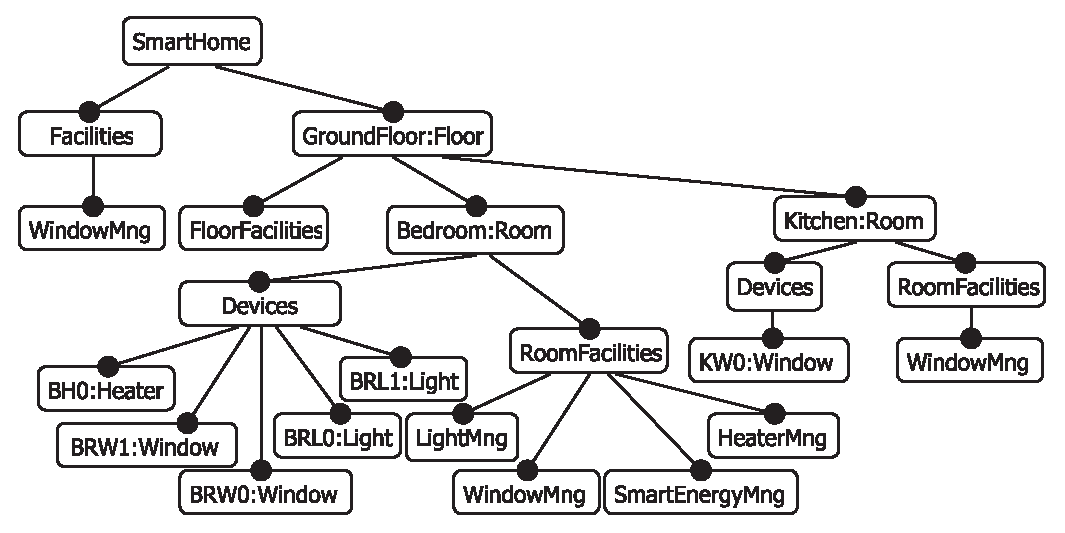
\includegraphics[width=\linewidth]{figures/configuration.eps} \\
  \caption{Configuration of a specific automated house}
  \label{fig:smartHomeCfg}
\end{figure*}

%============================================================================================
% NOTE(Pablo): Probably this is not interesting in any version of the paper
%============================================================================================
%
% In this case, the process has been as follows: (1) we have create a clone for the \imp{Floor} % feature; and we have called it \imp{GroundFloor}. (2) We have removed the \imp{Floor} feature % as more clones were not required; (3) Similarly, we have created two clones of the \imp{Room} % feature, one for the \imp{Kitchen} and other one for the {Bedroom}. The subtree
% below Room was cloned and copied below the \imp{Kitchen} and \imp{Bedroom} features. (4) 
% Then, we have created clones for the devices which must be placed in each room according to 
% the user requirements. (5) Finally, we have selected the \imp {WindowMng} facility for the 
% entire house; all the facilities for the \imp{Bedroom}; and no extra facilities, beyond \imp
% {WindowMng}, for the \imp{Kitchen}. We have not defined any facility at the \imp{Floor} 
% level.
%
%============================================================================================

%============================================================================================
% NOTE(Pablo): This has been removed for the sake of simplicity
%============================================================================================
%
% This feature model makes also use of another advanced mechanisms for feature modelling, which % are \emph{feature references}~\cite{czarnecki:2005}. A feature reference is a feature that 
% references another feature. In Figure~\ref{fig:smartHomeFM}, \imp{FloorFacilities} and 
% \imp{RoomFacilities} are feature references. Both them refer to \imp{Facilities} (this 
% relationship is not explicitly displayed in the diagram). The semantics of a feature 
% reference is to replace the feature reference with the subtree with root in the feature that % is referenced. In our case, \imp{FloorFacilities} and \imp{RoomFacilities} would be replaced % with the subtree with root in \imp{Facilities}. Feature references help to avoid redundancies % in feature models, which contributes to scalability.
%
%============================================================================================

Nevertheless, clonable features creates new challenges when the specification of cross-tree constraints is required. For instance, according to Figure~\ref{fig:smartHomeFM}, house facilities can be selected at a house, floor or room level. Therefore, a cross-tree constraint should specify if \imp{LightMng} has been selected at the floor level, this facility must also have been selected for each room belonging to that floor.

Since \imp{SmartEnergyMng} requires the \imp{HeaterMng} and \imp{WindowMng} features have been selected, other constraint should specify whenever \imp{SmartEnergyMng} has been selected at one level (e.g. for a specific floor), \imp{HeaterMng} and \imp{WindowMng} have also been selected at the same level (i.e. for that specific floor). Moreover, we might want to specify more advanced constraints, like if \imp{Presence Simulation} is going to be included in a automated house, at least a 30\% of the rooms in the house must include automatic light management.

In feature models, the most usual way to express cross-tree constraints is using propositional logic formulas, like \imp{SmartEnergyMng implies (LightMng and HeaterMng)}, where the different features are the atoms for these formulas~\cite{batory:2005}. A feature is evaluated to true when it has been selected, and false otherwise. The main problem when dealing with clonable features is that this correspondence is not useful anymore. Clonable features are not selected or unselected, they are simply cloned. So, the meaning of a atom related to clonable feature becomes undefined and, as a result, the formula can not be evaluated.     








\subsection{Research challenges on clonable features}

%============================================================================%
% Author: Pablo S�nchez                                                      %
%         p.sanchez@unican.es, http://personales.unican.es/sanchezbp         %
% Section : Research Challenges                            Date: 25/02/2011  %
% Version : 1.0                                                              %
% Conference: SPLC 2011                                                      %
%============================================================================%

%============================================================================================
% NOTE(Pablo): This is not required for SPLC 2011
%============================================================================================
%
% The creation of clonable features was initially an easy task, since it only required to add
% the notion of cardinality to each feature. Nevertheless, this has created several
% side-effects, since some concepts such as the semantics of a clonable feature selection, had % to be reviewed and updated. This section identifies several problems, not currently solved to % the best of our knowledge, regarding the specification of external constraints involving
% clonable features.
%
%============================================================================================

%============================================================================================
% NOTE(Pablo): Too much verbose
%============================================================================================
%
% Nevertheless, this had several consequences, since it was required to review an update
% well-established concepts related to feature modelling and to answer several research
% challenges that emerged as a consequence of introducing this new concept. Previous section
% described how clonable features are selected by means of a new cloning operation. This
% section identifies several problems, not currently solved to the best of our knowledge,
% regarding the specification of external constraints between features when some of the
% features involved in the constraint are clonable.
%
%============================================================================================

Clonable features creates new challenges when the specification of cross-tree constraints is required. For instance, according to Figure~\ref{fig:smartHomeFM}, house facilities can be selected at a house, floor or room level. Therefore, a cross-tree constraint should specify if \imp{LightMng} has been selected at the floor level, this facility must also have been selected for each room belonging to that floor.

Since \imp{SmartEnergyMng} requires the \imp{HeaterMng} and \imp{WindowMng} features have been selected, other constraint should specify whenever \imp{SmartEnergyMng} has been selected at one level (e.g. for a specific floor), \imp{HeaterMng} and \imp{WindowMng} have also been selected at the same level (i.e. for that specific floor). Finally, we might want to specify more advanced constraints, like if \imp{Presence Simulation} is going to be included in a automated house, a 25\% of the rooms in the house at least must include automatic light management .

In feature models, the most usual way to express cross-tree constraints is using propositional logic formulas, such as \imp{SmartEnergyMng implies (LightMng and HeaterMng)}, where the different features are the atoms for these formulas~\cite{batory:2005}. An atom is evaluated to true when the corresponding feature has been selected, otherwise it is false. The main problem when dealing with clonable features is that this correspondence cannot be used. Clonable features are not selected or unselected. Clonable are just cloned. So, the meaning of a atom related to a clonable feature becomes undefined. As a result, a propositional logical formula including clonable features can not be evaluated and it can not be determined when the corresponding constraint has been satisfied or violated.

For instance, let us suppose  \imp{A} and \imp{B} are clonable features. In this case, what would be the meaning of a external constraint like \imp{A implies B}? Does this means that one instance of \imp{A} implies the existence of at least one instance of \imp{B}? Or, on the other hand, does it means that the existence of all potential \imp{A}s implies the existence of all potential \imp{B}s? Or, why not, the existence of all potential \imp{A}s implies the existence of only one \imp{B}? So, the first research challenge we face is to decide what a clonable feature exactly means in a logical formula expressing a cross-tree constraint.

Each clonable feature really evaluates to a set of clones. For instance, the feature \imp{Floor} in Figure~\ref{fig:smartHomeFM} actually evaluates to \imp{\{Ground, First \}}, instead of selected or unselected. Thus, we might want to specify properties that only applies to: (1) at least one element in that set (e.g. only to the \imp{Ground} floor); (2) to all the elements in that set that fulfill a certain constraint (e.g to all the floors with \imp{LightMng} selected in one room at least); or (3) all the elements in the set. This would allow us to express more complex constraints such as, such as: if \imp{HeaterMng} is selected per house level, one \imp{Room} at least must contain one \imp{Heater} as a minimum. So, our second research challenge is to add quantification mechanisms to constraints involving clonable features.

%============================================================================================
% TODO(Pablo): Redo this image using Hydra. It is quite hard to get Hydra working for this
%              purpose
%============================================================================================

\begin{figure}[!tb]
  % Requires \usepackage{graphicx}
  \centering 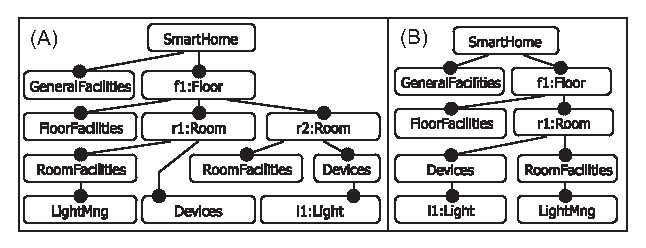
\includegraphics[width=\linewidth]{Figures/contexts.eps} \\
  \caption{(Left) Invalid configuration (Right) Valid configuration}
  \label{fig:contexts}
\end{figure}

Moreover, as already commented in previous section, we might want to specify constraints which must be evaluated for a particular subtree of the whole feature model, i.e. in a particular \emph{context}. For instance, if \imp{LightMng} has been selected for a particular \imp{Room}, such a \imp{Room} must have one \imp{Light} at least. Thus, we should specify a constraint like ``\imp{LightMng} implies one \imp{Light} device at least''. If we do not limit the scope in which this constraint is evaluated, this constraint will be true for the configurations of Figure~\ref{fig:contexts} (a) and (b). Nevertheless, this constraint should be false for Figure~\ref{fig:contexts} (a), since \imp{r1:Room} has selected the \imp{LightMng} facility, but it has not any \imp{Light} device to control. This means this constraint must be evaluated for all rooms (notice we are using again quantification) and using only the subtree below each \imp{Room}. Thus, the third research challenge is how to specify and analyse constraints which must be must be evaluated in the scope of a particular context.

%============================================================================================
% NOTE(Pablo): Since we have opted for leaving out feature references, this paragraph must
%              also be left out of the paper.
%============================================================================================
%
% Contexts are also useful for solve ambiguities when using feature references, since multiple % copies of a same feature might appear at different part of a configuration model. For
% instance, does \imp{LightMng} refers to \imp{LightMng} for \imp{GeneralFacilities},
% \imp{FloorFacilities} or \imp{RoomFacilities}. Using contexts, we can limit the scope of a
% name to unambiguously refer to a certain feature.
%
%============================================================================================

Finally, we would to like to point out that not only clonable features can have more than one instance per configuration of a feature model. All those features that have as an ancestor a clonable features can appear more than once in a configuration model. We will call to this kind of feature, i.e. non clonable features with a clonable ancestor, \emph{multiple features}.
Figure~\ref{fig:multipleFtr} illustrates this situation.In this case, the feature \imp{LightMng} below \imp{RoomFacilities} appears two times due to the \imp{Room} feature has been cloned twice. This implies that \imp{LightMng}, as well as the other features below \imp{Room}, also evaluate to a set of features instead of simply to true or false. Nevertheless, it should be noticed that these multiple features, oppositely to clonable features, can be evaluated to true or false if they are evaluated in a particular context.
For example, the \imp{LightMng} feature in Figure~\ref{fig:multipleFtr} can be evaluated to true or false when it is evaluated in the context of a particular room. So, our last research challenge is how to deal appropriately with \emph{multiple features}.

\begin{figure}[!tb]
  \centering 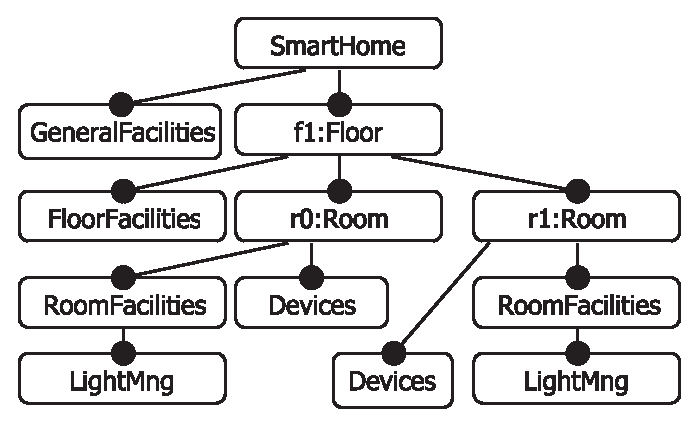
\includegraphics[width=.65\linewidth]{Figures/multipleFeatures.eps} \\
  \caption{The \emph{multiple features} phenomena}
  \label{fig:multipleFtr}
\end{figure}

Summarising, when dealing with clonable features, we should to address the following research challenges to properly express and analyse cross-tree constraints between features:

\begin{enumerate}
	\item What a clonable feature means in a cross-tree constraint.
	\item Add quantification mechanisms to cross-tree constraints.
	\item Add the notion of \emph{context} to cross-tree constraints.
	\item Manage properly multiple features.
\end{enumerate}

To the best of our knowledge, there is currently no research work, and consequently no tool, addressing these challenges. To overcome this limitation, we have firstly created a language for expressing arbitrary complex constraints including clonable features as a stepping stone towards the analysis of constraints including clonable (or multiple) features. Next section describes sauch a language.

%============================================================================================
% NOTE(Pablo) : This have been supressed because it sounds redundant
%============================================================================================
%
% We have implemented a reasoner able to decide if a set of external constraints, involving
% clonable or multiple features, is satisfied given a specific configuration of a feature
% model. The reasoner is also able to perform some extra task, such as deciding which features % must be incorporated to a configuration in order to satisfy the external constraints. We have % integrated this language and the reasoner in our feature modelling environment, which we have % called \emph{Hydra}.
%
%============================================================================================

%============================================================================================
% NOTE(Pablo) : We have reduced this paragraph. We are no presenting a tool, so this
%               paragraph can be simply skipped
%============================================================================================
%
% State-of-art tools only offer two operators, \imp{implies} and \imp{excludes}, and deal with % simple propositional formulas. This is clearly not enough to address the research challenges % described in this section.
%
%============================================================================================

%=============================================================================================
% NOTE(Pablo): This paragraph would be suitable for a very general venue                                                                                 %=============================================================================================
%
% A typical feature modelling process would be as follows:
%
% \begin{enumerate}
%    \item First of all, a feature model is created. A feature model is a tree representation
%          of the features included in % a set of products and of the relationships between
%          them.
%    \item Since not all the relationships between features can be captured using simply the
%          syntax provided by feature  models, it is often required to specify some external
%          constraints, which restrict the way in which features in a feature model can be
%          selected. For instance, we might specify that if a certain feature \imp{A} is
%          selected, another feature \imp{B} can not be selected, due to a bad interaction
%          between these features.
%    \item Once we have created a feature model, we can use it for creating configurations,
%          i.e. selection of features that specify which particular features are, or it will
%          be, included in a certain product.
%    \item To ensure we are creating correct configurations, we need to validate that a
%          configuration obeys the rules the % syntax of the feature model, and, in addition,
%          it also satisfies the external defined constraints.
% \end{enumerate}
%
%=============================================================================================

 